\documentclass[]{beamer}
\usepackage[T1]{fontenc}
\usepackage[utf8]{inputenc}
\usepackage{lmodern}
\usepackage[italian]{babel}

\title{Il linguaggio HTML}
\author{\texorpdfstring{Mattia Cozzi\newline\href{mailto:cozzimattia@gmail.com}{\texttt{cozzimattia@gmail.com}}}{Mattia Cozzi}}
\date{a.s.~2023/2024}


%\documentclass[handout]{beamer}     %usare questa classe per generare l'handout

%\usepackage{pdfpages}   %per mostrare più quadri nella stessa pagina
%\pgfpagesuselayout{4 on 1}[a4paper,border shrink=5mm,landscape]


\usetheme{Singapore}
%\useoutertheme[left]{sidebar} %elementi intorno alle diapositive
\setbeamercovered{dynamic} %modifica l'aspetto del testo grigetto delle diapositive future. Argomenti: invisible/transparent/dynamic

%COLORE PRINCIPALE
\definecolor{verde}{RGB}{2, 194, 117} % UBC Blue (primary)
\setbeamercolor{structure}{fg=verde} % itemize, enumerate, etc
\setbeamercolor{alerted text}{fg=verde}


\usecolortheme{orchid}

\usepackage{tikz}

\begin{document}

\begin{frame}
  \titlepage
\end{frame}


\begin{frame}
\frametitle{Contenuti}
\tableofcontents
\end{frame}

\section{Introduzione}


\begin{frame}
\frametitle{Navigare}
Quando navighiamo sul web apriamo diverse \alert<1-3>{pagine} con il nostro browser.

\begin{columns}
\begin{column}{0.5\textwidth}
\begin{figure}
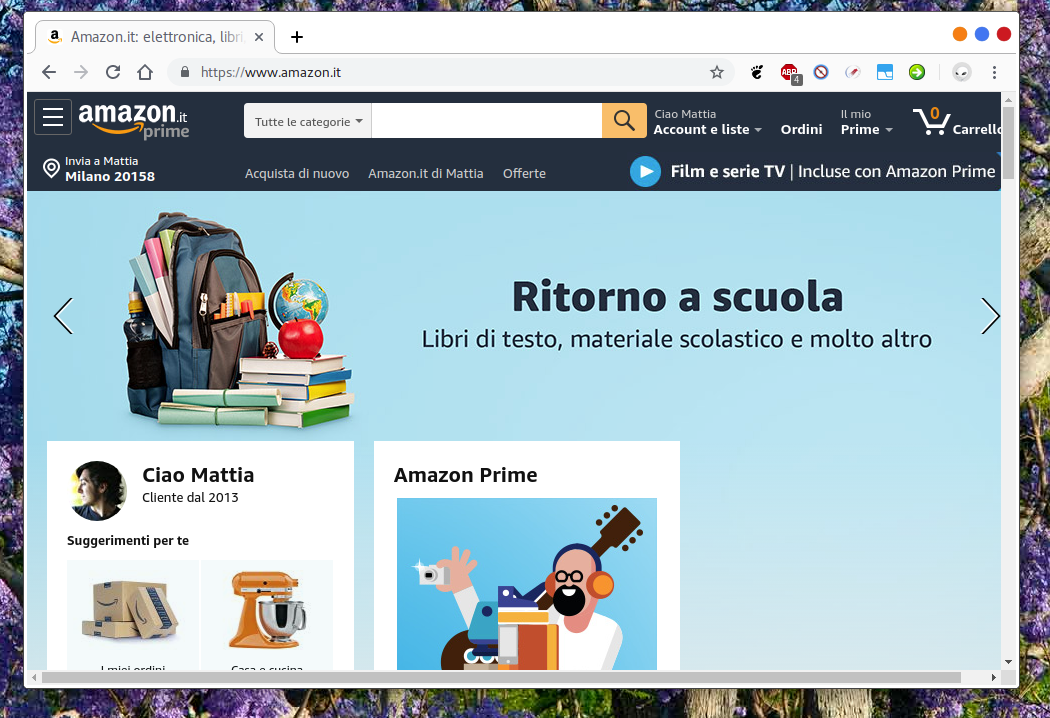
\includegraphics[width=\columnwidth]{screenshots/chrome.png}
\end{figure}
\end{column}
\begin{column}{0.2\textwidth}
\visible<2->{\begin{figure}

\includegraphics[width=\columnwidth]{screenshots/chromemobile.jpg}
\end{figure}}
\end{column}
\begin{column}{0.2\textwidth}
\visible<3->{\begin{figure}

\includegraphics[width=\columnwidth]{screenshots/safari.png}
\end{figure}}
\end{column}
\end{columns}\pause\pause\pause

~

~

Ma cosa è una pagina web?
\end{frame}

\begin{frame}
\frametitle{Documenti HTML (1)}
Quando apriamo una pagina web, il nostro browser richiede al server un \alert{file in formato \texttt{.html}}.
\begin{figure}

\includegraphics[width=.8\columnwidth]{screenshots/html.png}
\end{figure}
\end{frame}


\begin{frame}
\frametitle{Documenti HTML (2)}
\begin{columns}
\begin{column}{0.6\textwidth}
\begin{figure}
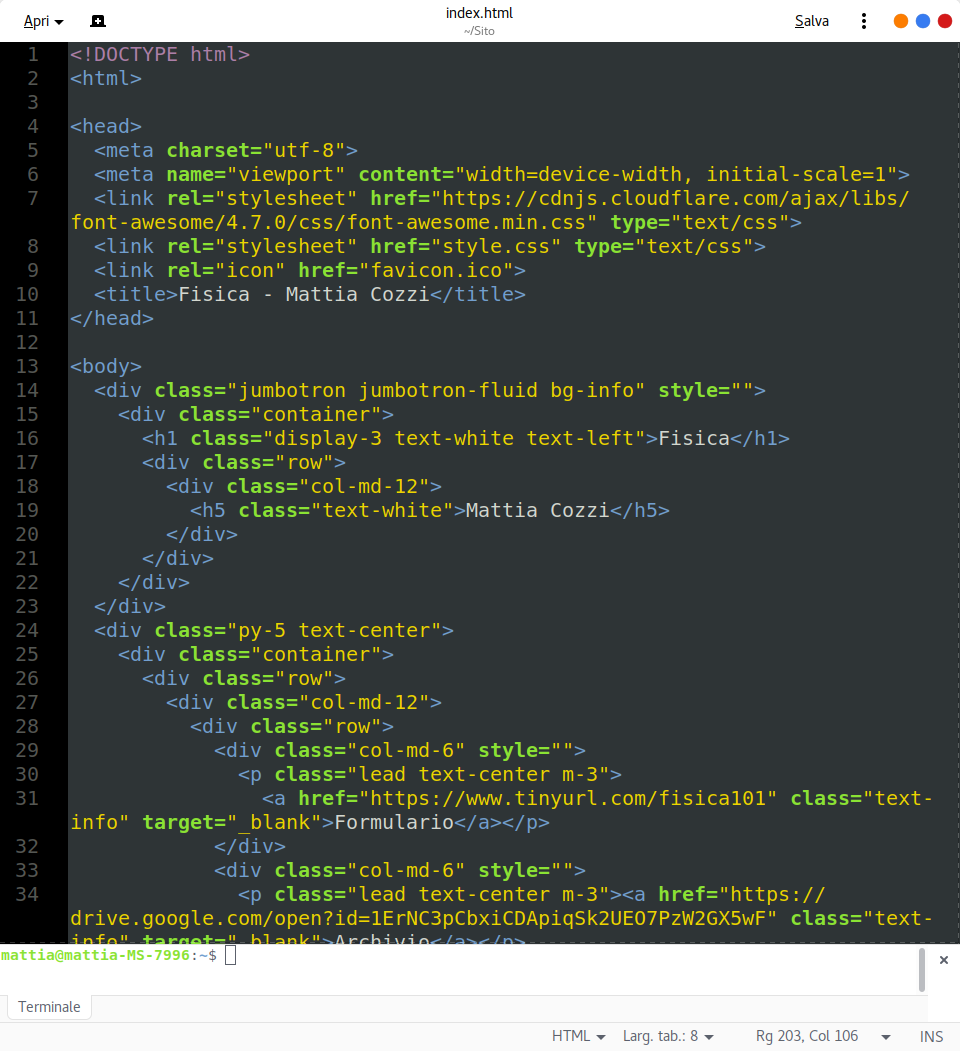
\includegraphics[width=\columnwidth]{screenshots/testosemplice.png}
\end{figure}
\end{column}
\begin{column}{0.3\textwidth}
I file \texttt{.html} sono file di \alert{testo semplice}, editabile anche con un semplice blocco note.

~

Questo testo è il \alert{codice HTML}, scritto in un apposito linguaggio.
\end{column}
\end{columns}
\end{frame}



\begin{frame}
\frametitle{Documenti HTML (3)}
Un browser (come Google Chrome o Safari):\pause
\begin{itemize}
  \item apre un file HTML;\pause
  \item ne legge il codice;\pause
  \item lo interpreta graficamente;\pause
  \item mostra all'utente la pagina formattata.\pause
\end{itemize}
\vspace*{-.7cm}
\begin{columns}
\begin{column}{0.45\textwidth}
\begin{figure}
\visible<6>{\fbox{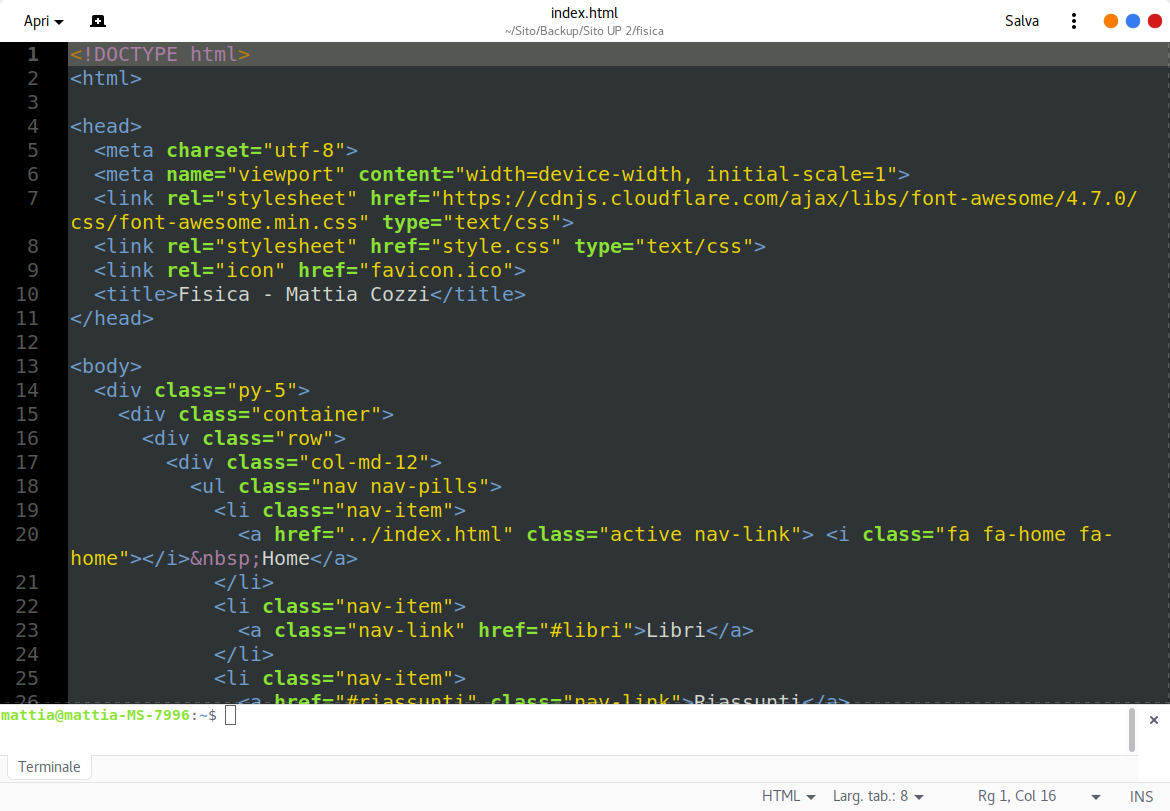
\includegraphics[width=\columnwidth]{screenshots/sitotesto.png}}}
\end{figure}
\end{column}
\begin{column}{0.45\textwidth}
\begin{figure}
\visible<6>{\fbox{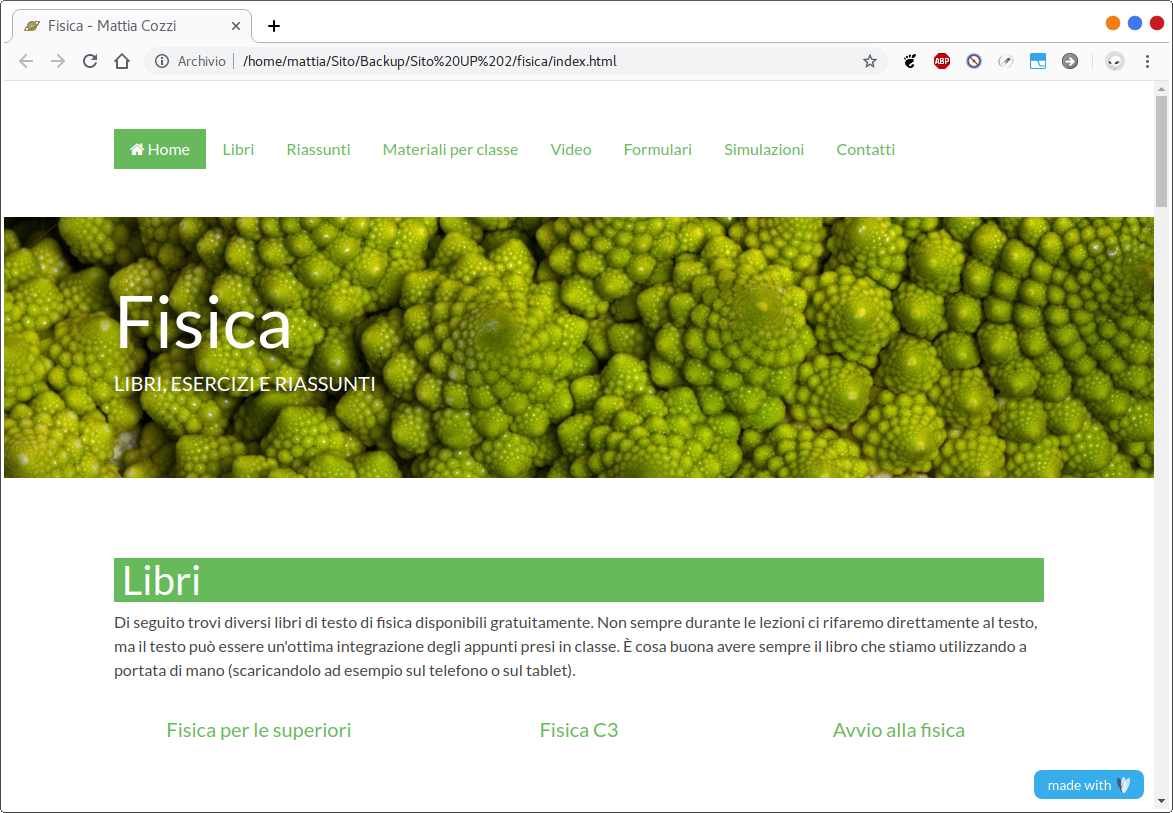
\includegraphics[width=\columnwidth,]{screenshots/sitoformattato.png}}}
\end{figure}
\end{column}
\end{columns}
\end{frame}



\begin{frame}
\frametitle{Visualizzare il codice sorgente di una pagina}
Tutti i browser desktop permettono di visualizzare il codice HTML della pagina che si sta visualizzando:\pause
\begin{itemize}
  \item con il mouse, click destro in un punto vuoto della pagina, ``Visualizza sorgente pagina'';
\begin{figure}
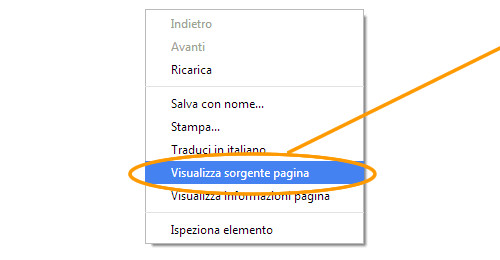
\includegraphics[width=.6\columnwidth]{screenshots/sorgente.jpg}
\end{figure}\pause
  \item con la tastiera, \colorbox{black}{\textcolor{white}{CTRL}} + \colorbox{black}{\textcolor{white}{U}}.
\end{itemize}
\end{frame}


\begin{frame}
\frametitle{Creare e modificare del codice}
Sebbene per HTML basti un blocco note, possiamo anche usare un \alert<1>{editor dedicato}.\pause

~

Vantaggi:
\begin{itemize}
  \item aprire più file contemporaneamente grazie alle \alert<2->{schede};\pause
  \item leggere meglio il codice grazie al \alert<3->{syntax highlighting};\pause
  \item navigare agevolmente il codice grazie ai \alert<4->{numeri di riga};\pause
  \item velocizzare la scrittura grazie all'\alert<5->{autocompletamento}.
\end{itemize}
\end{frame}

\begin{frame}
\frametitle{Editor proposti (open source)}
\begin{figure}

\includegraphics[width=.7\columnwidth]{screenshots/vscode.png}

\href{https://code.visualstudio.com/download}{\texttt{https://code.visualstudio.com/}}
\end{figure}

~

\begin{figure}

\includegraphics[width=.7\columnwidth]{screenshots/atom.png}

\href{https://atom.io/}{\texttt{https://atom.io/}}
\end{figure}
\end{frame}


\begin{frame}
\frametitle{Modalità di lavoro}
Imparare il codice HTML richiede molte prove, molti errori e molte verifiche.\pause

~

Workflow:
\begin{enumerate}
  \item aprire il file html con Atom/VS Code (click destro sul file, ``Apri con...'');\pause
  \item aprire lo stesso file html con un browser (doppio click sul file);\pause
  \item scrivere/modificare il file in Atom/VS Code;\pause
  \item salvare le modifiche (\colorbox{black}{\textcolor{white}{CTRL}} + \colorbox{black}{\textcolor{white}{S}});\pause
  \item ricaricare la pagina nel browser (\colorbox{black}{\textcolor{white}{F5}} oppure \colorbox{black}{\textcolor{white}{CTRL}} + \colorbox{black}{\textcolor{white}{R}});\pause
  \item verificare il risultato.
\end{enumerate}
\end{frame}

\begin{frame}
\frametitle{Problemi di spazio}
Dovendo passare (e pensare) spesso da una finestra all'altra, una disposizione classica delle finestre risulta scomoda.
\begin{figure}
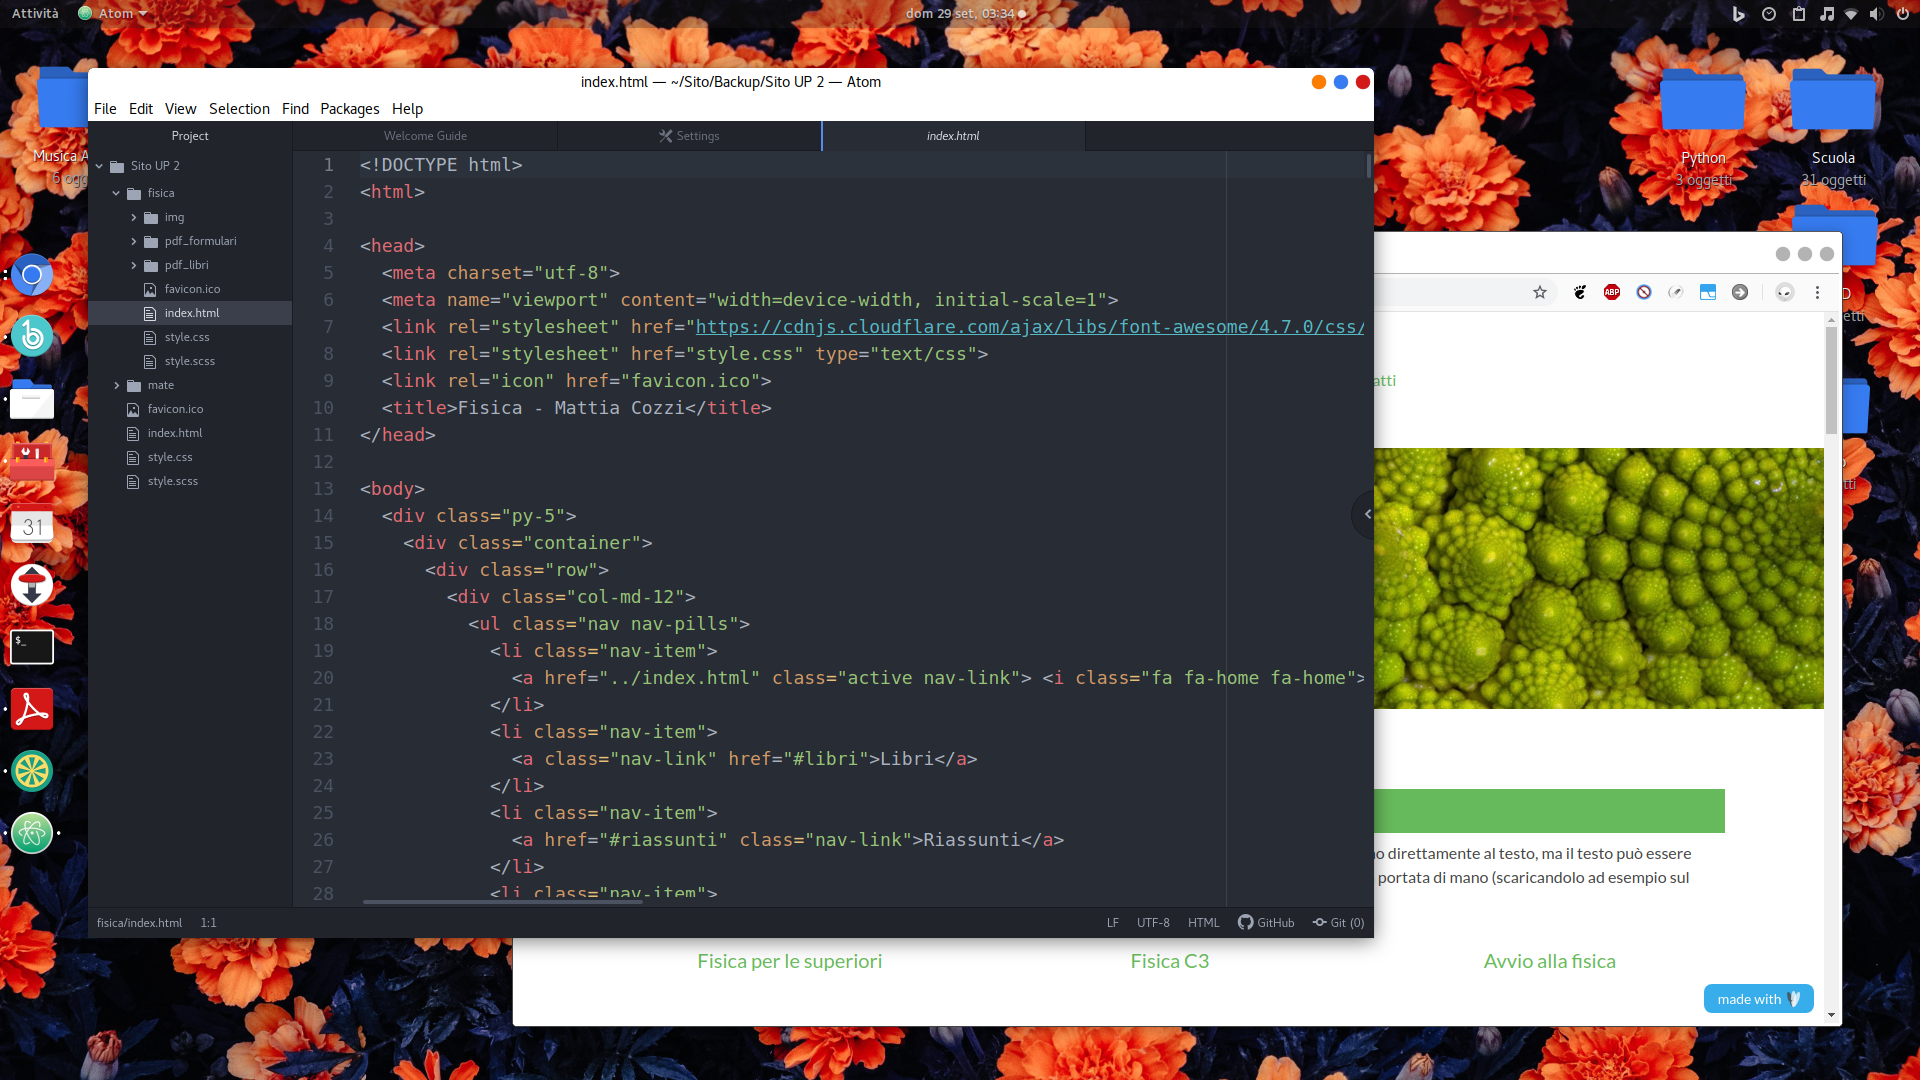
\includegraphics[width=.9\columnwidth]{screenshots/workflow1.png}
\end{figure}
\end{frame}


\begin{frame}
\frametitle{Migliorare il workflow con il \emph{tiling}}

Su Windows, possiamo affiancare due finestre con \colorbox{black}{\textcolor{cyan}{WIN}} \textcolor{cyan}{+} \colorbox{black}{$ \textcolor{cyan}{\rightarrow} $} e \colorbox{black}{\textcolor{magenta}{WIN}} \textcolor{magenta}{+} \colorbox{black}{$ \textcolor{magenta}{\leftarrow} $}.

\begin{figure}
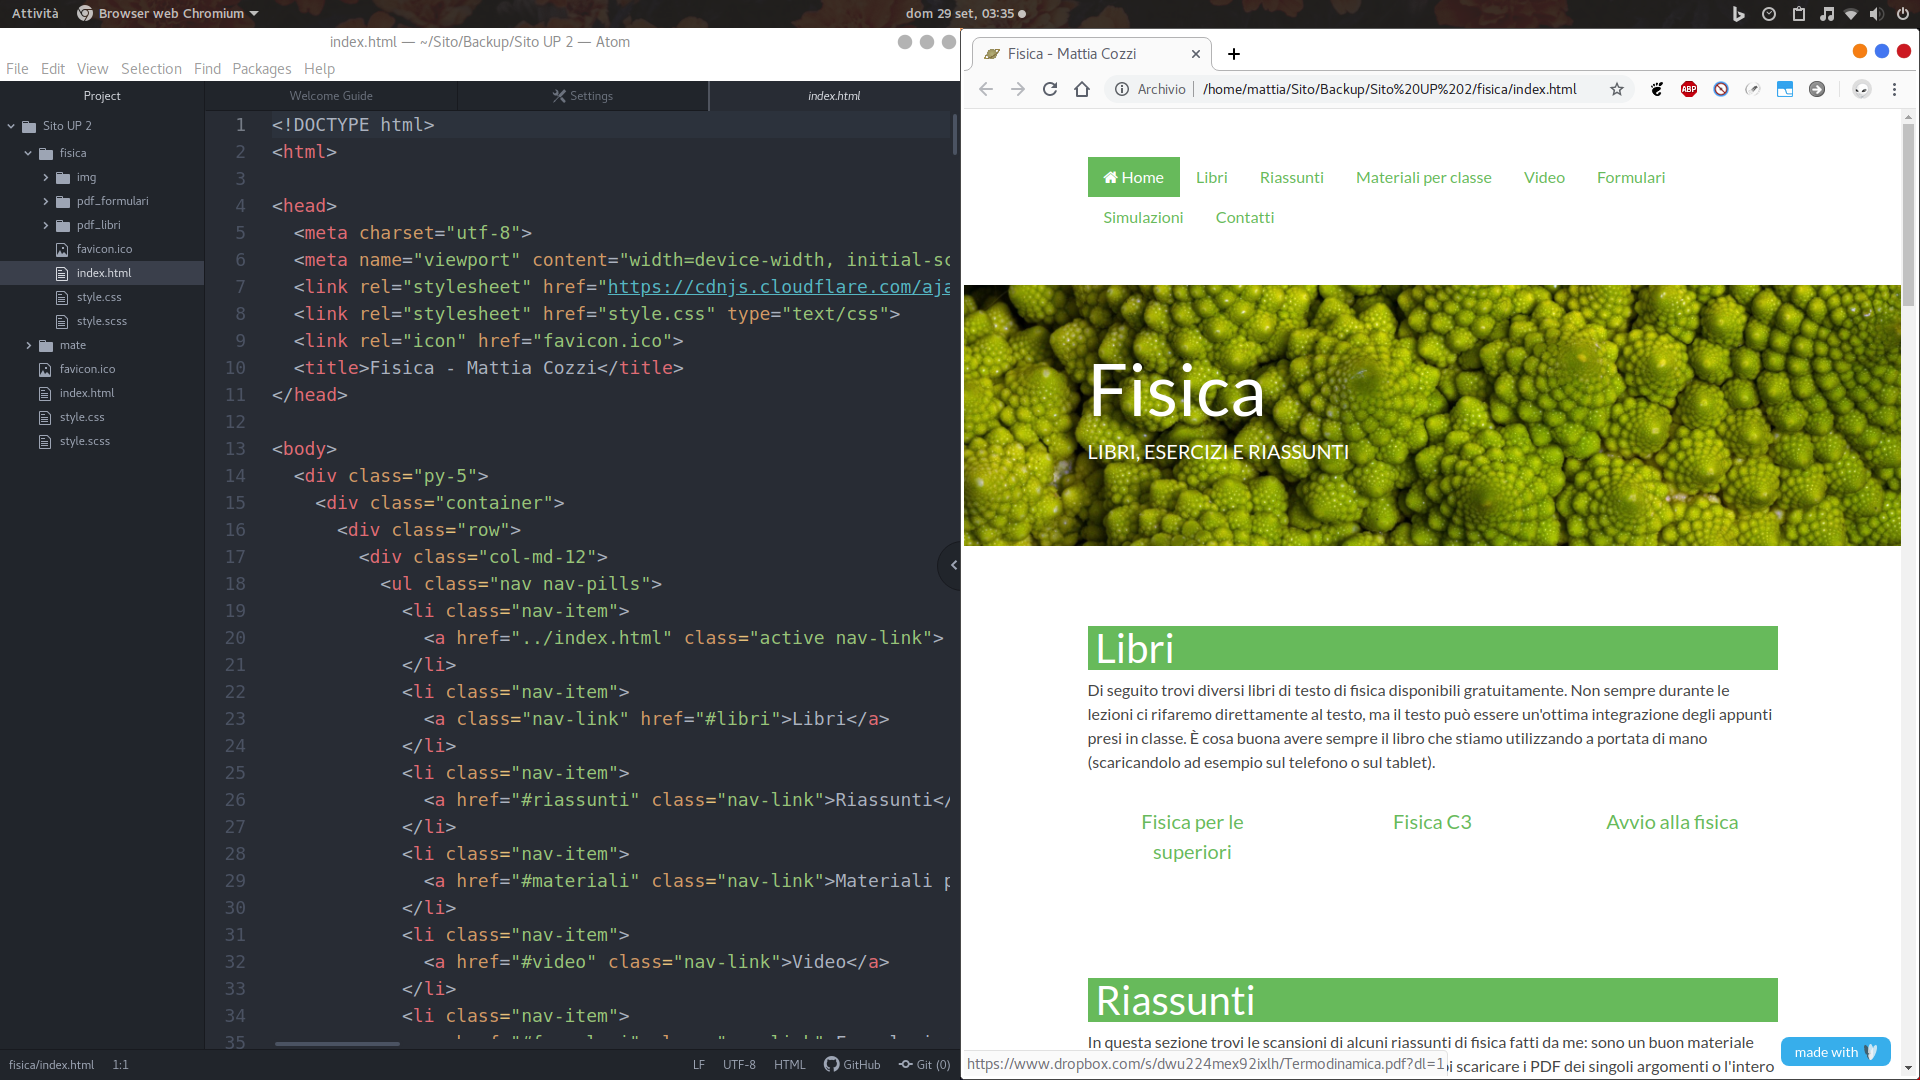
\includegraphics[width=.9\columnwidth]{screenshots/workflow2.png}
\end{figure}


\end{frame}




\section{Tag}


\begin{frame}
\frametitle{Linguaggio}
Attenzione: \alert<1>{HTML non è un linguaggio di programmazione!}\pause

~

HTML è l'acronimo di \alert<2>{\emph{HyperText Markup Language}} (linguaggio di contrassegno per gli ipertesti).

Ipertesti = documenti collegati da link.\pause

~

È  un linguaggio di markup che indica \alert<3>{come disporre gli elementi} all'interno della pagina.
\end{frame}

\begin{frame}
\frametitle{Marcatori}
La disposizione viene indicata attraverso dei \alert<1>{tag} (``etichette'').\pause

~

I tag sono riconoscibili perché sono indicati tra \alert<2>{parentesi angolari}.

\begin{figure}
\visible<2>{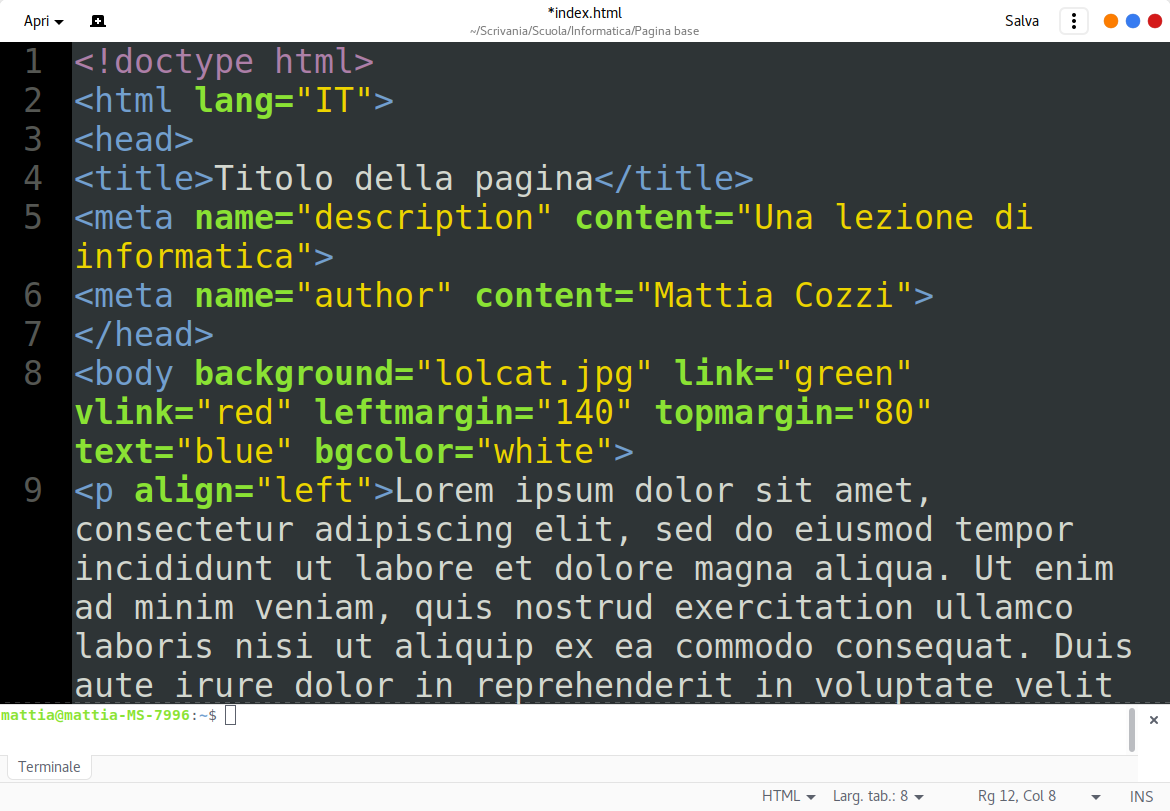
\includegraphics[width=.7\columnwidth]{screenshots/tag.png}}
\end{figure}
\end{frame}

\begin{frame}
\frametitle{Sintassi dei tag}
Un tag HTML è quasi sempre un \alert<1>{contenitore}.\pause

~

\begin{itemize}
  \item \texttt{\textcolor{magenta}{<h1>}I mammiferi marini\textcolor{magenta}{</h1>}}
  
  ~
  
  \item \texttt{\textcolor{cyan}{<p>}Lorem ipsum dolor sit amet, consectetur adipiscing elit, sed do eiusmod tempor incididunt ut labore et dolore magna aliqua. Ut enim ad minim veniam, quis nostrud exercitation ullamco laboris nisi ut aliquip ex ea commodo consequat.\textcolor{cyan}{</p>}}
\end{itemize}

~

\pause
I tag possono essere quindi \alert<3>{aperti} e \alert<3>{chiusi}.
\end{frame}



\begin{frame}[fragile]
\frametitle{Indentazione}
Scriveremo spesso dei tag all'interno di altri tag. Per migliorare la leggibilità, è bene lasciare dello spazio all'inizio di una riga.
\begin{columns}
\begin{column}{0.5\textwidth}
\begin{scriptsize}
\begin{verbatim}
<html>
  <head>
    <title>Tazze</title>
  </head>
  <body>
    <h1>Offerte</h1>
    <p>Sfoglia il volantino con
    tutte le promozioni.</p>
  </body>
</html>
\end{verbatim}
\end{scriptsize}\pause
\end{column}
\begin{column}{0.3\textwidth}
\begin{figure}
\visible<2>{
\includegraphics[width=\columnwidth]{screenshots/tab.png}}
\end{figure}
\end{column}
\end{columns}  
\end{frame}

\begin{frame}[fragile]
\frametitle{Gli attributi}
I tag possono essere accompagnati da uno o più attributi, che specificano caratteristiche del tag.

\begin{center}
\texttt{<\textcolor{magenta}{tag} \textcolor{cyan}{attributo1}=''\textcolor{orange}{valore1}'' \textcolor{cyan}{attributo2}=''\textcolor{orange}{valore2}''>}
\end{center}\pause


~

Esempio:
\begin{center}
{\small \texttt{<body leftmargin="30px" text="yellow" bgcolor="black">}}
\end{center}
\end{frame}















\section{Head e body}

\begin{frame}
\frametitle{DocType}
Un file HTML inizia solitamente con una \emph{dichiarazione DocType}.\pause

~

Questa riga informa il browser circa il tipo di documento che andrà ad interpretare.\pause

~

Ha forma:
\begin{center}
\texttt{<!DOCTYPE html>}
\end{center}
\end{frame}

\begin{frame}[fragile]
\frametitle{Intestazione e corpo}
Tutto il contenuto della pagina web è scritto all'interno del tag \alert<1>{\texttt{html}}.\pause
  
~
  
Il contenuto è poi diviso tra il tag \alert<2>{\texttt{head}} e il tag \alert<2>{\texttt{body}}.

\begin{columns}
\begin{column}{0.2\textwidth}
\begin{scriptsize}
\begin{verbatim}
  <html>
    <head>
      ...
    </head>
    <body>
      ...
    </body>
  </html>
\end{verbatim}
\end{scriptsize}\pause
\end{column}
\begin{column}{0.7\textwidth}

\begin{itemize}
  \item \alert<3>{\texttt{head}} contiene metadati sulla pagina (titolo, autore, script, ecc.);\pause
  
  ~
  
  \item \alert<4>{\texttt{body}} contiene la pagina vera e propria (testo, immagini, tabelle, video, ecc.).
\end{itemize}
\end{column}
\end{columns}  
\end{frame}


\begin{frame}[fragile]
\frametitle{Contenuti del tag \texttt{head}}
\begin{itemize}
  \item Titolo della pagina:
  \begin{center}
  \alert<1>{\texttt{<title>Titolo della pagina</title>}}\pause
  \end{center}
  ~
\begin{columns}
\begin{column}{0.5\textwidth}
\begin{scriptsize}
\begin{verbatim}
<head>
<title>Lezione di informatica</title>
</head>
\end{verbatim}
\end{scriptsize}
\end{column}
\begin{column}{0.3\textwidth}
\visible<2->{\begin{figure}

\includegraphics[width=\columnwidth]{screenshots/titolo.png}
\end{figure}}
\end{column}
\end{columns}\pause
~

~
  \item Autore della pagina:
  \begin{center}
  \alert<3>{\texttt{<meta name=''author'' content=''Dante Alighieri''>}}
  \end{center}~\pause
  \item Descrizione della pagina:
  \begin{center}
  \alert<4>{\texttt{<meta name=''description'' content=''\ldots''>}}
  \end{center}
\end{itemize}
\end{frame}




\begin{frame}[fragile]
\frametitle{Commenti}
Sono parti di testo che vengono ignorate dal browser. 

~

Utili per chiarire il codice all'autore stesso e al lettore.\pause
  
~
  
Sintassi:
\begin{center}
\texttt{<!{-}{-} testo del commento {-}{-}>}
\end{center}

\end{frame}


\begin{frame}[fragile]
\frametitle{Corpo del documento}
Il tag \texttt{body} ha i seguenti attributi:
\begin{description}
    \item[Margini] In pixel, \texttt{leftmargin=n} e \texttt{topmargin=n}\pause
    \item[Colore testo] \texttt{text="white"}\\(il colore può anche essere indicato in RGB)\pause
    \item[Colore link] \texttt{link="blue"} per i link non visitati, \texttt{vlink="yellow"} per i visitati\pause
    \item[Col sfondo] \texttt{bgcolor="black"}\pause
    \item[Img sfondo] \texttt{background="file.jpg"}\pause
    \item[Sfondo fisso] \texttt{bgproperties="fixed"}
  \end{description}
\end{frame}




\begin{frame}[fragile]
\frametitle{Esempio}
\visible<1->{
\begin{center}
\texttt{<body leftmargin="30px" topmargin="30px" text="yellow" bgcolor="black">}
\end{center}}

\begin{figure}
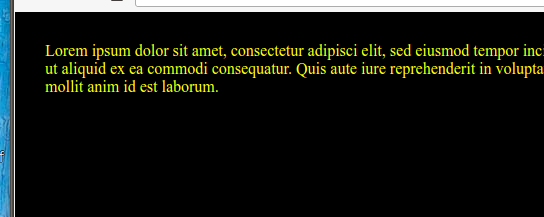
\includegraphics[width=.7\columnwidth]{screenshots/corpo.png}
\end{figure}
\end{frame}


\section{Divisione}

\begin{frame}[fragile]
\frametitle{Paragrafo}
I paragrafi (tag \texttt{p}) \alert<1>{raggruppano del testo}, mandando a capo alla chiusura del tag.\pause

~

Il tag \texttt{p} \alert<2>{inserisce dello spazio prima e dopo} il blocco di testo.\pause

~

Può essere indicato l'\alert<3>{allineamento}: \texttt{left}, \texttt{right}, \texttt{center}, \texttt{justify}.\pause
\visible<4->{\begin{columns}
\begin{column}{0.45\textwidth}
\begin{tiny}
\texttt{~\\
<p align="center">Lorem ipsum dolor sit amet, consectetur adipisci ...</p>\newline
<p align="right">Ut enim ad minim veniam, quis nostrum exercitationem ...</p>
}
\end{tiny}
\end{column}
\begin{column}{0.45\textwidth}
\begin{figure}
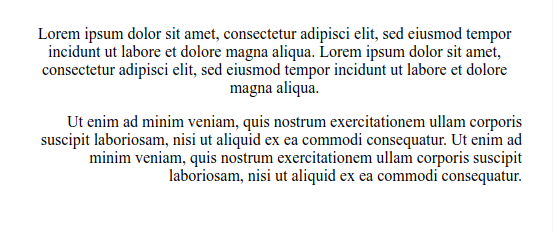
\includegraphics[width=\columnwidth]{screenshots/paragrafo.png}
\end{figure}
\end{column}
\end{columns}}
\end{frame}



\begin{frame}[fragile]
\frametitle{Divisione}
Il tag \texttt{div} è simile al tag \texttt{p}, ma \alert<1>{non lascia spazio} prima e dopo il blocco di testo.\pause

~

Può essere indicato l'\alert<2>{allineamento}: \texttt{left}, \texttt{right}, \texttt{center}, \texttt{justify}.\pause
\visible<3->{\begin{columns}
\begin{column}{0.45\textwidth}
\begin{tiny}
\texttt{~\\
<div align="center">Lorem ipsum dolor sit amet, consectetur adipisci ...</div>\newline
<div align="right">Ut enim ad minim veniam, quis nostrum exercitationem ...</div>
}
\end{tiny}
\end{column}
\begin{column}{0.45\textwidth}
\begin{figure}
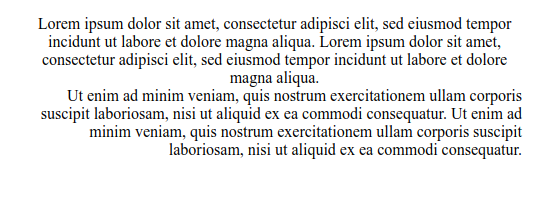
\includegraphics[width=\columnwidth]{screenshots/divisione.png}
\end{figure}
\end{column}
\end{columns}}
\end{frame}

\begin{frame}[fragile]
\frametitle{Andare a capo}
Notiamo che se mandiamo a capo nell'editor, il testo nel browser non va comunque a capo.

~

Per mandare del testo a capo \alert{senza chiudere un paragrafo o una divisione}, si può usare il \emph{tag vuoto} \texttt{<br />} o \texttt{<br>} (break line).\pause

\visible<3->{\begin{columns}
\begin{column}{0.4\textwidth}
\begin{tiny}
\texttt{~\\
<p>Lorem ipsum dolor<br>sit amet,\newline<br>consectetur adipisci</p>
}
\end{tiny}
\end{column}
\begin{column}{0.4\textwidth}
\begin{figure}

\includegraphics[width=.5\columnwidth]{screenshots/acapo.png}
\end{figure}
\end{column}
\end{columns}}
\end{frame}



\begin{frame}[fragile]
\frametitle{Linea di separazione}
Anche questo è un tag vuoto: \texttt{<hr />} (horizontal line). Ammette diversi attributi:\visible<2->{
  \begin{description}
    \item[Allineamento] \texttt{align="center/right/left"} 
    \item[Larghezza] \texttt{width="20px/50\%"} 
    \item[Spessore] \texttt{size="2px/10\%"}
    \item[Colore] \texttt{color="red"}  
    \item[Ombra] \texttt{noshade} 
  \end{description}
}

\visible<3->{\begin{columns}
\begin{column}{0.45\textwidth}
\begin{tiny}
\texttt{~\\
<p>Lorem ipsum dolor sit amet...\newline
<hr  width="50px" color="red" size="3px" />\newline
Ut enim ad minim veniam, quis...</p>
}
\end{tiny}
\end{column}
\begin{column}{0.45\textwidth}
\begin{figure}
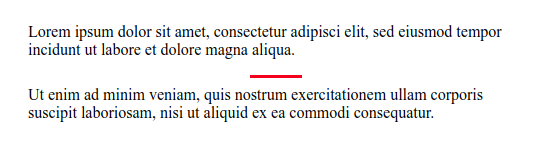
\includegraphics[width=\columnwidth]{screenshots/linea.png}
\end{figure}
\end{column}
\end{columns}}
\end{frame}




\section{Testo}

\begin{frame}[fragile]
\frametitle{Stile del testo (1)}
La sintassi generale per formattare una certa parte di testo è:
\begin{center}
\texttt{<font attributo="valore">testo</font>}
\end{center}

\visible<2->{
\begin{description}
    \item[Font] \texttt{face="courier-times new roman-verdana"} 
    \item[Dimensione] \texttt{size="5"}, dove il numero può essere da 1 a 7 per le dimensioni assolute (default 3) o da -7 a +7 per le dimensioni relative
    \item[Colore] \texttt{color="red"}
  \end{description}
}

\visible<3->{\begin{columns}
\begin{column}{0.45\textwidth}
\begin{tiny}
\texttt{~\\
<font face="courier" color="red">Testo1</font>\newline
<font face="verdana" color="blue">Testo2</font>
}
\end{tiny}
\end{column}
\begin{column}{0.45\textwidth}
\begin{figure}

\includegraphics[width=.7\columnwidth]{screenshots/font.png}
\end{figure}
\end{column}
\end{columns}}
\end{frame}




\begin{frame}[fragile]
\frametitle{Stile del testo (2)}
Possiamo anche rendere il testo \textbf{grassetto}, \textit{corsivo}, \underline{sottolineato} o in altro modo, semplicemente racchiudendo del testo in un apposito tag.

\visible<2->{\begin{columns}
\begin{column}{0.45\textwidth}
\begin{tiny}
\texttt{~\\
<b>Attenzione</b> <i>a non</i> <u>esagerare</u> <s>con tutti</s> <tt>i possibili</tt> <sup>stili</sup> <sub>del testo</sub>!
}
\end{tiny}
\end{column}
\begin{column}{0.45\textwidth}
\begin{figure}

\includegraphics[width=\columnwidth]{screenshots/stili.png}
\end{figure}
\end{column}
\end{columns}}
\end{frame}



\begin{frame}[fragile]
\frametitle{Titoli}
Possiamo formattare una certa parte di testo come titolo (o sottotitolo) con la sintassi:
\begin{center}
\texttt{<hN align="left/center/right">Titolo</hN>}
\end{center}
con N compreso tra 1 e 6.

\visible<2->{\begin{columns}
\begin{column}{0.45\textwidth}
\begin{tiny}
\texttt{~\\
<h1 align="left">Titolo 1</h1>\newline
<h2 align="left">Titolo 2</h2>\newline
<h3 align="left">Titolo 3</h3>\newline
<h4 align="left">Titolo 4</h4>
}
\end{tiny}
\end{column}
\begin{column}{0.45\textwidth}
\begin{figure}
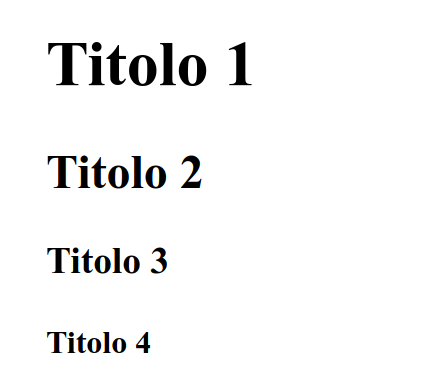
\includegraphics[width=.7\columnwidth]{screenshots/titoli.png}
\end{figure}
\end{column}
\end{columns}}
\end{frame}




\section{Immagini}

\begin{frame}[fragile]
\frametitle{Immagini}
\visible<1->{
Per inserire immagini si usa il tag senza chiusura:

\begin{center}
\texttt{<img src="file.jpg">}
\end{center}}
\visible<2->{
\begin{description}
    \item[Bordo] \texttt{border="2px"}
    \item[Larghezza] \texttt{width="30\%"}
    \item[Altezza] \texttt{height="50px"}
    \item[Testo alt] \texttt{alt="Testo"}
  \end{description}
}
\visible<3->{\begin{columns}
\begin{column}{0.5\textwidth}
\begin{scriptsize}
\texttt{~\\
<img src="tempio.jpg" width="50\%">
}
\end{scriptsize}
\end{column}
\begin{column}{0.4\textwidth}
\begin{figure}
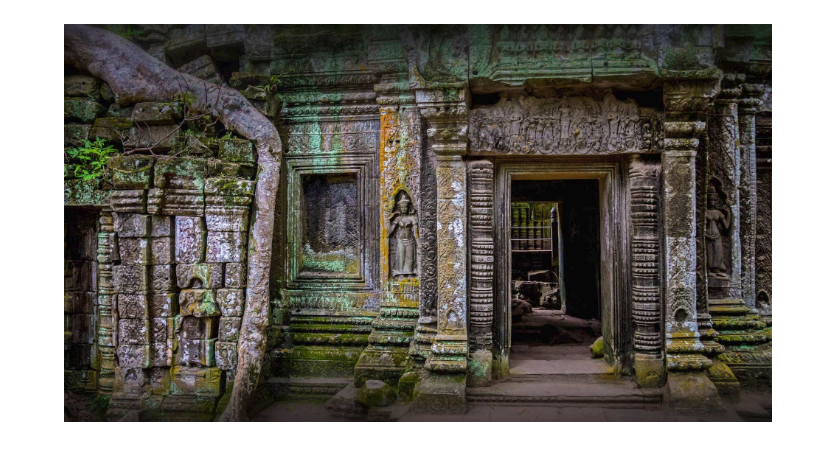
\includegraphics[width=\columnwidth]{screenshots/immagine.png}
\end{figure}
\end{column}
\end{columns}}
\end{frame}

\begin{frame}[fragile]
\frametitle{Path (percorso) delle immagini}
Quando un sito contiene molte immagini, è comodo e utile organizzarle in cartelle.\pause

La cartella attuale si indica con \texttt{./}, quella superiore con \texttt{../}.
  
  
  
\visible<3->{\begin{columns}
\begin{column}{0.5\textwidth}
{\footnotesize Nella pagina \texttt{index.html} scriveremo:}\\
\begin{tiny}
\texttt{
~\\
<img src="./img/cartella1/immagine1.jpg">\\
<img src="./img/cartella2/immagine6.jpg">
}
\end{tiny}
\end{column}
\begin{column}{0.4\textwidth}
\begin{figure}
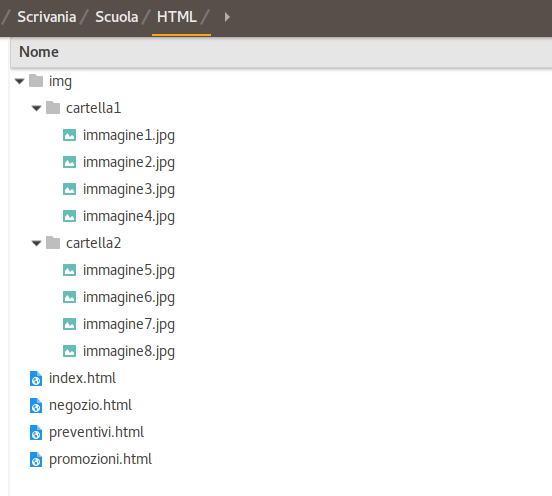
\includegraphics[width=\columnwidth]{screenshots/albero.png}
\end{figure}
\end{column}
\end{columns}}
  
  
\end{frame}






\section{Elenchi}


\begin{frame}[fragile]
\frametitle{Elenchi puntati}
\texttt{ul} = unordered list, \texttt{li} = list item.
\begin{columns}
\begin{column}{0.45\textwidth}
\begin{scriptsize}
\begin{verbatim}
<ul type="disc"> <!-- default -->
  <li>Primo
  <li>Secondo
  <li>Terzo
</ul>

<ul type="circle">
  <li>Primo
  <li>Secondo
  <li>Terzo
</ul>

<ul type="square">
  <li>Primo
  <li>Secondo
  <li>Terzo
</ul>
\end{verbatim}
\end{scriptsize}
\end{column}
\begin{column}{0.45\textwidth}
\begin{figure}
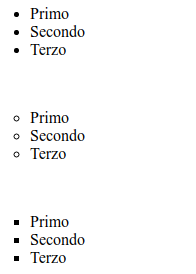
\includegraphics[width=0.5\columnwidth]{screenshots/elencopuntato.png}
\end{figure}
\end{column}
\end{columns}
\end{frame}



\begin{frame}[fragile]
\frametitle{Elenchi numerati (1)}
\texttt{ol} = ordered list, \texttt{li} = list item.
\begin{columns}
\begin{column}{0.45\textwidth}
\begin{scriptsize}
\begin{verbatim}
<ol type="1"> <!-- default -->
  <li>Primo
  <li>Secondo
  <li>Terzo
</ol>

<ol type="I">
  <li>Primo
  <li>Secondo
  <li>Terzo
</ol>

<ol type="i">
  <li>Primo
  <li>Secondo
  <li>Terzo
</ol>
\end{verbatim}
\end{scriptsize}
\end{column}
\begin{column}{0.45\textwidth}
\begin{figure}
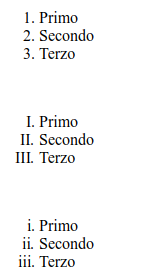
\includegraphics[width=0.4\columnwidth]{screenshots/elenconumerato1.png}
\end{figure}
\end{column}
\end{columns}
\end{frame}




\begin{frame}[fragile]
\frametitle{Elenchi numerati (2)}

\begin{columns}
\begin{column}{0.45\textwidth}
\begin{scriptsize}
\begin{verbatim}
<ol type="A">
  <li>Primo
  <li>Secondo
  <li>Terzo
</ol>

<ol type="a">
  <li>Primo
  <li>Secondo
  <li>Terzo
</ol>
\end{verbatim}
\end{scriptsize}
\end{column}
\begin{column}{0.45\textwidth}
\begin{figure}
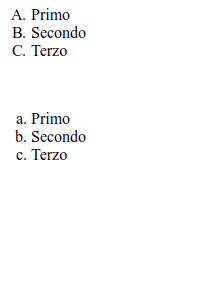
\includegraphics[width=0.5\columnwidth]{screenshots/elenconumerato2.png}
\end{figure}
\end{column}
\end{columns}
\end{frame}







\begin{frame}[fragile]
\frametitle{Elenchi di definizioni}
\texttt{dl} = definition list.
\begin{columns}
\begin{column}{0.45\textwidth}
\begin{scriptsize}
\begin{verbatim}
<dl>
<dt>Gatto<dd>Felino da compagnia
<dt>Canarino<dd>Volatile da compagnia
<dt>Criceto<dd>Roditore da compagnia
</dl>
\end{verbatim}
\end{scriptsize}
\end{column}
\begin{column}{0.45\textwidth}
\begin{figure}
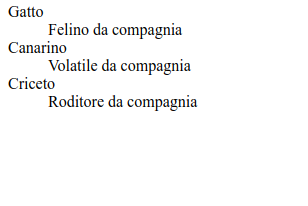
\includegraphics[width=0.8\columnwidth]{screenshots/definizioni.png}
\end{figure}
\end{column}
\end{columns}
\end{frame}


\section{Link}

\begin{frame}[fragile]
\frametitle{Link}
I link ad altre risorse (pagine HTML, media, punti della stessa o di un'altra pagina, ecc.) possono essere introdotti con la sintassi:
\begin{center}
\texttt{<a href="contatti.html">Scrivimi!</a>}
\end{center}

\visible<2->{Attributi:
\begin{description}
    \item[Titolo link] \texttt{title="titolo"}
    \item[Apertura] \texttt{target="\_new/blank"}
  \end{description}
}
\visible<3->{\begin{columns}
\begin{column}{0.6\textwidth}
\begin{scriptsize}
\texttt{~\\
<a href="contatti.html" \newline
title="Scrivi a Mattia">Scrivimi!</a>
}
\end{scriptsize}
\end{column}
\begin{column}{0.3\textwidth}
\begin{figure}

\includegraphics[width=\columnwidth]{screenshots/link.png}
\end{figure}
\end{column}
\end{columns}}
\end{frame}

\begin{frame}[fragile]
\frametitle{Etichette (1)}
Sono delle ancore senza testo e fungono da segnaposto a certi punti della pagina.
\begin{center}
\texttt{<a name="etichetta"></a>}
\end{center}

\visible<2->{Le etichette della pagina attuale (o di altre pagine) possono essere richiamate con la sintassi:
\begin{center}
\texttt{<a href="\#etichetta">testo</a>}\\
\texttt{<a href="./pagina2/\#etichetta">testo</a>}
\end{center}
}
\end{frame}



\begin{frame}[fragile]
\frametitle{Etichette (2)}
\visible<1->{Le etichette possono essere usate per creare un \emph{indice della pagina}.}
\visible<2->{\begin{columns}
\begin{column}{0.65\textwidth}
\begin{scriptsize}
\texttt{~\\
<a href="\#sezione1">Vai alla sezione 1</a><br>\newline
<a href="\#sezione2">Vai alla sezione 2</a><br>\newline
<a href="\#sezione3">Vai alla sezione 3</a>
}
\end{scriptsize}
\end{column}
\begin{column}{0.3\textwidth}
~\\~\\
\begin{figure}
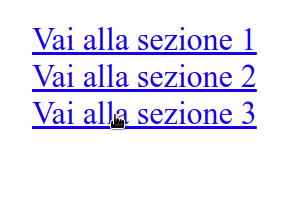
\includegraphics[width=\columnwidth]{screenshots/indice.png}
\end{figure}
\end{column}
\end{columns}}
\end{frame}



\section{Tabelle}

\begin{frame}[fragile]
\frametitle{Tabelle}
Le tabelle sono aperte e chiuse dal tag:
\begin{center}
\texttt{<table>...</table>}
\end{center}
che ammette i seguenti attributi:
  \begin{description}
    \item[Allineamento orizzontale] \texttt{align="left/center/right"}
    \item[Allineamento verticale] \texttt{valign="top/middle/bottom"}
    \item[Bordo della tabella] \texttt{border="1px"}
    \item[Larghezza e altezza] \texttt{width="30\%"} e \texttt{height="100px"} 
    \item[Spaziatura tra le celle] \texttt{cellspacing="5px"}
    \item[Spaziatura tra bordo e contenuto] \texttt{cellpadding="10px"}
    \item[Colore sfondo] \texttt{bgcolor="red"}
    \item[Immagine sfondo] \texttt{background="sfondo.jpg"}
  \end{description}
\end{frame}




\begin{frame}[fragile]
\frametitle{Righe e colonne}
Le righe sono indicate con \texttt{<tr>...</tr>} e ammettono l'attributo \texttt{height}, \texttt{bgcolor}, \texttt{background}, \texttt{align} e \texttt{valign}.\\~\\\pause


Le colonne sono indicate con \texttt{<td>...</td>} (\texttt{<th>} per l'header della tabella) e ammettono l'attributo \texttt{width}, oltre ai precedenti.
\end{frame}



\begin{frame}[fragile]
\frametitle{Esempio 1}

\begin{scriptsize}
\texttt{~\\
<table border="1px">\newline
<tr> <th>Uccelli con la T</th> <th>Uccelli con la P</th></tr>\newline
<tr align="right"> <td>Tordo</td> <td>Piccione</td></tr>\newline
<tr align="center"> <td>Tucano</td> <td>Pinguino</td></tr>\newline
<tr> <td>Tacchino</td> <td>Picchio</td></tr>\newline
</table>
}
\end{scriptsize}

\begin{figure}
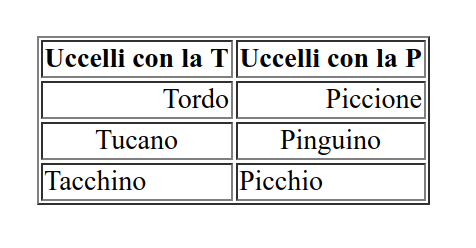
\includegraphics[width=.5\columnwidth]{screenshots/tabella1.png}
\end{figure}

\end{frame}






\begin{frame}[fragile]
\frametitle{Unire righe e colonne}
È possibile unire più celle orizzontalmente lavorando sulla cella corrispondente con la sintassi \texttt{<td colspan=2>}.\\~\\\pause
È possibile unire più celle verticalmente lavorando sulla cella corrispondente con la sintassi \texttt{<td rowspan=2>}.
\end{frame}




\begin{frame}[fragile]
\frametitle{Esempio 2}

\begin{scriptsize}
\texttt{~\\
<table border="1px">\newline
<tr> <th>Genere</th> <th>CD</th> <th>mp3</th> <th>Concerti</th></tr>\newline
<tr> <td rowspan=2>Musica folk</td> <td colspan=3>Angelo</td></tr>\newline
<tr> <td>458</td> <td>1125</td> <td>5</td></tr>\newline
<tr> <td rowspan=2>Musica pop</td> <td colspan=3>Fiorella</td></tr>\newline
<tr> <td>782</td> <td>1657</td> <td>3</td></tr>\newline
</table>
}
\end{scriptsize}

\begin{figure}
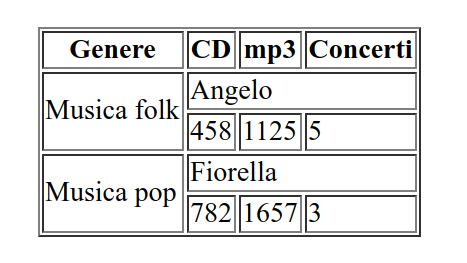
\includegraphics[width=.5\columnwidth]{screenshots/tabella2.png}
\end{figure}

\end{frame}


\end{document}
